Erste Beobachtungen der Effekte von Dunkler Materie wurden von Fritz Zwickey im Jahr 1933 gemacht.
Unter Verwendung des Virialsatzes der Thermodynamik berechnete er die Rotantionsgeschwindigkeit von Galaxien im Coma Cluster basierend auf der leuchtenden Materie.
Diese verglich er mit den über die Rotverschiebung bestimmten Rotationsgeschwindigkeiten und fand, dass die Masse ungefähr um eine $400$ faches kleiner ist als erwartet.\cite{Zwicky1933}
Um die Diskrepanz zu erklären postulierte er weitere nicht leuchtende Materie, Dunkle Materie.
Bis Heute wurden zahlreiche weitere Beobachtungen der Effekte von DM gemacht.
Erwartet wird, dass die gesamte Materie zu $\SI{84}{\percent}$\cite{Adam2016} aus DM besteht.
Im Folgenden werden die prominentesten dieser Beobachtungen vorgestellt.

\begin{figure}[!b]
\begin{center}
\includegraphics[width=0.8\textwidth]{./fig/Rubin80.pdf}
\end{center}
\caption{Rotationsgeschwindigkeit in Abhängigkeit des Radius zum Zentrum für 21 Sc Galaxien.\cite{Rubin80}}
\label{fig:Rubin21Sc}
\end{figure}

\subsection*{Rotationskurven von Galaxien}
Für die Rotationsgeschwindigkeit von Galaxien erwarten wir anhand der newtonschen Mechanik
\begin{equation}
v(R) = \sqrt{\frac{GM(R)}{R}}
\label{eq:Keppler}
\end{equation}
hier ist $G$ die Gravitationskonstante, $R$ der Abstand zum Zentrum der Rotation und $M(R)$ die gesamte Massen innerhalb einer Kugel des Radius $R$ um das Zentrum.  
Ab einem gewissen Abstand ist der Großteil der sichtbaren Masse von dieser Kugel eingeschlossen.
Ab dann bleibt $M(R)$ ungefähr konstant und die Rotationsgeschwindigkeit nimmt mit $1/\sqrt{R}$ ab.
Dieses verhalten wurde mittels Rotverschiebung von Vera Rubin in den 70er Jahren anhand von Spiralgalaxien untersucht.
Mit dem Ergebnis, dass die Rotationskurven aller von ihr untersuchten Galaxien konstant bleiben oder sogar ansteigen weit jenseits ihrer größten Leuchtkraft, siehe Abbildung \ref{fig:Rubin21Sc}.
Dies suggeriert eine nicht leuchtende, linear mit dem Radius ansteigende Massenverteilung.\cite{Rubin80}
Jüngste Beobachtungen zeigen, dass auch Galaxie mit fast keiner DM auftreten können\cite{VanDokkum2018}.
Dunkle Materie und Baryonische Materie sind daher nicht immer aneinander gekoppelt wie es für Theorien wie MOND\cite{1983ApJ...270..365M} (\textit{Modified Newtonian dynamics}) und emergent gravity paradigm\cite{Verlinde2016} notwendig ist in denen die Effekte Dunkle Materie eine Konsequenz Baryonischer Materie sind.

\begin{figure}[!b]
\begin{center}
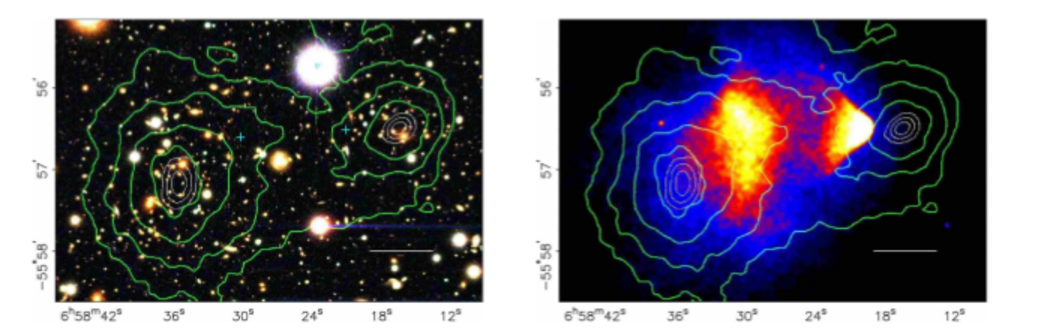
\includegraphics[width=\textwidth]{./fig/Bullet.pdf}
\end{center}
\caption{Links:Aufnahme des Bullet Cluster vom Magellan Teleskop.
Rechts: Röntgenaufnahme des Bullet Cluster vom Chandra Teleskop.
Die Konturen zeigen die durch den schwachen Gravitationslinseneffekt erwartete Massenverteilung.\cite{Clowe2006}}
\label{fig:BulletC}
\end{figure}

\subsection*{Evidenz aus Gravitationslinseneffekten}
Als Gravitationslinseneffekt wird die Ablenkung von Licht durch die Raumkrümmung massereicher Objekte bezeichnet und führt dazu, dass Objekte vergrößert, verzerrt oder heller erscheinen\cite{Massey2010}.
Mittels des schwachen Gravitationslinseneffekt wurde außergewöhnliche Erkenntnisse über die Massenverteilung im Bullet Cluster gewonnen.
Das Bullet Cluster besteht aus zwei kollidierten Clustern.
Bei der Kollision sind die Galaxien der Cluster fast ungehindert passiert.
Der Großteil der Clustermassen in Form von interstellarem Gas befindet sich allerdings noch im Zentrum der Kollision und erzeugt Röntegnstrahlung auf Grund Elektromagnetischer Wechselwirkungen, in Abb. \ref{fig:BulletC} links dargestellt.
Die durch den schwachen Gravitationslinseneffekt bestimmte Massenverteilung zeigt allerdings weitere um die ursprünglichen Cluster verteilte Materie welche bei der Kollision kaum wechselwirkte.
Aus der Position des warmen Gas und der Position der Dunklen Materie kann die Größe der Selbstwechselwirkung von Dunkler Materie eingeschränkt werden.\cite{Markevitch2003}
